\documentclass[twoside]{book}

% Packages required by doxygen
\usepackage{fixltx2e}
\usepackage{calc}
\usepackage{doxygen}
\usepackage[export]{adjustbox} % also loads graphicx
\usepackage{graphicx}
\usepackage[utf8]{inputenc}
\usepackage{makeidx}
\usepackage{multicol}
\usepackage{multirow}
\PassOptionsToPackage{warn}{textcomp}
\usepackage{textcomp}
\usepackage[nointegrals]{wasysym}
\usepackage[table]{xcolor}

% Font selection
\usepackage[T1]{fontenc}
\usepackage[scaled=.90]{helvet}
\usepackage{courier}
\usepackage{amssymb}
\usepackage{sectsty}
\renewcommand{\familydefault}{\sfdefault}
\allsectionsfont{%
  \fontseries{bc}\selectfont%
  \color{darkgray}%
}
\renewcommand{\DoxyLabelFont}{%
  \fontseries{bc}\selectfont%
  \color{darkgray}%
}
\newcommand{\+}{\discretionary{\mbox{\scriptsize$\hookleftarrow$}}{}{}}

% Page & text layout
\usepackage{geometry}
\geometry{%
  a4paper,%
  top=2.5cm,%
  bottom=2.5cm,%
  left=2.5cm,%
  right=2.5cm%
}
\tolerance=750
\hfuzz=15pt
\hbadness=750
\setlength{\emergencystretch}{15pt}
\setlength{\parindent}{0cm}
\setlength{\parskip}{3ex plus 2ex minus 2ex}
\makeatletter
\renewcommand{\paragraph}{%
  \@startsection{paragraph}{4}{0ex}{-1.0ex}{1.0ex}{%
    \normalfont\normalsize\bfseries\SS@parafont%
  }%
}
\renewcommand{\subparagraph}{%
  \@startsection{subparagraph}{5}{0ex}{-1.0ex}{1.0ex}{%
    \normalfont\normalsize\bfseries\SS@subparafont%
  }%
}
\makeatother

% Headers & footers
\usepackage{fancyhdr}
\pagestyle{fancyplain}
\fancyhead[LE]{\fancyplain{}{\bfseries\thepage}}
\fancyhead[CE]{\fancyplain{}{}}
\fancyhead[RE]{\fancyplain{}{\bfseries\leftmark}}
\fancyhead[LO]{\fancyplain{}{\bfseries\rightmark}}
\fancyhead[CO]{\fancyplain{}{}}
\fancyhead[RO]{\fancyplain{}{\bfseries\thepage}}
\fancyfoot[LE]{\fancyplain{}{}}
\fancyfoot[CE]{\fancyplain{}{}}
\fancyfoot[RE]{\fancyplain{}{\bfseries\scriptsize Generated by Doxygen }}
\fancyfoot[LO]{\fancyplain{}{\bfseries\scriptsize Generated by Doxygen }}
\fancyfoot[CO]{\fancyplain{}{}}
\fancyfoot[RO]{\fancyplain{}{}}
\renewcommand{\footrulewidth}{0.4pt}
\renewcommand{\chaptermark}[1]{%
  \markboth{#1}{}%
}
\renewcommand{\sectionmark}[1]{%
  \markright{\thesection\ #1}%
}

% Indices & bibliography
\usepackage{natbib}
\usepackage[titles]{tocloft}
\setcounter{tocdepth}{3}
\setcounter{secnumdepth}{5}
\makeindex

% Hyperlinks (required, but should be loaded last)
\usepackage{ifpdf}
\ifpdf
  \usepackage[pdftex,pagebackref=true]{hyperref}
\else
  \usepackage[ps2pdf,pagebackref=true]{hyperref}
\fi
\hypersetup{%
  colorlinks=true,%
  linkcolor=blue,%
  citecolor=blue,%
  unicode%
}

% Custom commands
\newcommand{\clearemptydoublepage}{%
  \newpage{\pagestyle{empty}\cleardoublepage}%
}

\usepackage{caption}
\captionsetup{labelsep=space,justification=centering,font={bf},singlelinecheck=off,skip=4pt,position=top}

%===== C O N T E N T S =====

\begin{document}

% Titlepage & ToC
\hypersetup{pageanchor=false,
             bookmarksnumbered=true,
             pdfencoding=unicode
            }
\pagenumbering{alph}
\begin{titlepage}
\vspace*{7cm}
\begin{center}%
{\Large My Project }\\
\vspace*{1cm}
{\large Generated by Doxygen 1.8.13}\\
\end{center}
\end{titlepage}
\clearemptydoublepage
\pagenumbering{roman}
\tableofcontents
\clearemptydoublepage
\pagenumbering{arabic}
\hypersetup{pageanchor=true}

%--- Begin generated contents ---
\chapter{Hierarchical Index}
\section{Class Hierarchy}
This inheritance list is sorted roughly, but not completely, alphabetically\+:\begin{DoxyCompactList}
\item J\+Panel\begin{DoxyCompactList}
\item \contentsline{section}{translation\+Visualizaton\+G\+U\+I.\+Color\+Legend\+Panel}{\pageref{classtranslation_visualizaton_g_u_i_1_1_color_legend_panel}}{}
\item \contentsline{section}{translation\+Visualizaton\+G\+U\+I.\+Concordance\+Panel}{\pageref{classtranslation_visualizaton_g_u_i_1_1_concordance_panel}}{}
\item \contentsline{section}{translation\+Visualizaton\+G\+U\+I.\+Version\+Chosen\+Panel}{\pageref{classtranslation_visualizaton_g_u_i_1_1_version_chosen_panel}}{}
\end{DoxyCompactList}
\end{DoxyCompactList}

\chapter{Class Index}
\section{Class List}
Here are the classes, structs, unions and interfaces with brief descriptions\+:\begin{DoxyCompactList}
\item\contentsline{section}{\hyperlink{classtranslation_visualizaton_g_u_i_1_1_color_legend_panel}{translation\+Visualizaton\+G\+U\+I.\+Color\+Legend\+Panel} }{\pageref{classtranslation_visualizaton_g_u_i_1_1_color_legend_panel}}{}
\item\contentsline{section}{\hyperlink{classtranslation_visualizaton_g_u_i_1_1_concordance_panel}{translation\+Visualizaton\+G\+U\+I.\+Concordance\+Panel} }{\pageref{classtranslation_visualizaton_g_u_i_1_1_concordance_panel}}{}
\item\contentsline{section}{\hyperlink{classtranslation_visualizaton_g_u_i_1_1_version_chosen_panel}{translation\+Visualizaton\+G\+U\+I.\+Version\+Chosen\+Panel} }{\pageref{classtranslation_visualizaton_g_u_i_1_1_version_chosen_panel}}{}
\end{DoxyCompactList}

\chapter{Class Documentation}
\hypertarget{classtranslation_visualizaton_g_u_i_1_1_color_legend_panel}{}\section{translation\+Visualizaton\+G\+U\+I.\+Color\+Legend\+Panel Class Reference}
\label{classtranslation_visualizaton_g_u_i_1_1_color_legend_panel}\index{translation\+Visualizaton\+G\+U\+I.\+Color\+Legend\+Panel@{translation\+Visualizaton\+G\+U\+I.\+Color\+Legend\+Panel}}
Inheritance diagram for translation\+Visualizaton\+G\+U\+I.\+Color\+Legend\+Panel\+:\begin{figure}[H]
\begin{center}
\leavevmode
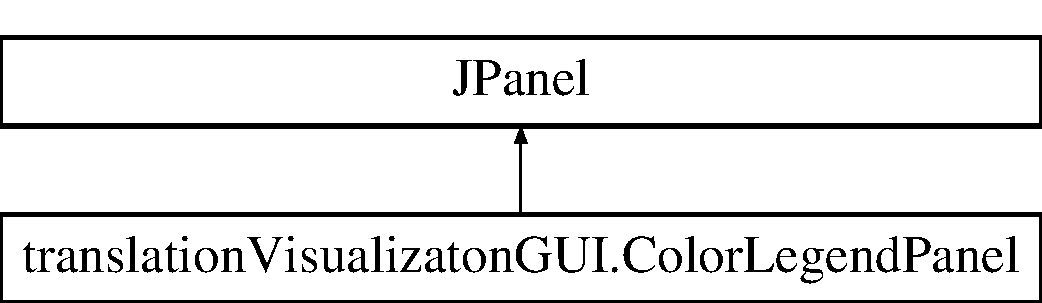
\includegraphics[height=2.000000cm]{classtranslation_visualizaton_g_u_i_1_1_color_legend_panel}
\end{center}
\end{figure}
\subsection*{Public Member Functions}
\begin{DoxyCompactItemize}
\item 
\mbox{\Hypertarget{classtranslation_visualizaton_g_u_i_1_1_color_legend_panel_abafc1059179fe94a5c6064981bc6474b}\label{classtranslation_visualizaton_g_u_i_1_1_color_legend_panel_abafc1059179fe94a5c6064981bc6474b}} 
Grid\+Bag\+Constraints {\bfseries get\+Constraint} ()
\item 
\mbox{\Hypertarget{classtranslation_visualizaton_g_u_i_1_1_color_legend_panel_ac712fb3754a75cfbc2490f0e00938c21}\label{classtranslation_visualizaton_g_u_i_1_1_color_legend_panel_ac712fb3754a75cfbc2490f0e00938c21}} 
\hyperlink{classtranslation_visualizaton_g_u_i_1_1_concordance_panel}{Concordance\+Panel} {\bfseries get\+M\+\_\+\+Concordance\+Panel} ()
\item 
\mbox{\Hypertarget{classtranslation_visualizaton_g_u_i_1_1_color_legend_panel_a35ec62b52c1530439f2b27ab6f34e603}\label{classtranslation_visualizaton_g_u_i_1_1_color_legend_panel_a35ec62b52c1530439f2b27ab6f34e603}} 
void {\bfseries set\+M\+\_\+\+Concordance\+Panel} (\hyperlink{classtranslation_visualizaton_g_u_i_1_1_concordance_panel}{Concordance\+Panel} m\+\_\+\+Concordance\+Panel)
\item 
\mbox{\Hypertarget{classtranslation_visualizaton_g_u_i_1_1_color_legend_panel_aa91c8659c551eba463ce5148241abf3a}\label{classtranslation_visualizaton_g_u_i_1_1_color_legend_panel_aa91c8659c551eba463ce5148241abf3a}} 
void {\bfseries set\+Color\+Legend} (List$<$ Map.\+Entry$<$ Integer, Color $>$$>$ m\+\_\+\+Color\+Index, List$<$ Map.\+Entry$<$ String, Integer $>$$>$ m\+\_\+\+Frequency\+Index)
\end{DoxyCompactItemize}


The documentation for this class was generated from the following file\+:\begin{DoxyCompactItemize}
\item 
Color\+Legend\+Panel.\+java\end{DoxyCompactItemize}

\hypertarget{classtranslation_visualizaton_g_u_i_1_1_concordance_panel}{}\section{translation\+Visualizaton\+G\+U\+I.\+Concordance\+Panel Class Reference}
\label{classtranslation_visualizaton_g_u_i_1_1_concordance_panel}\index{translation\+Visualizaton\+G\+U\+I.\+Concordance\+Panel@{translation\+Visualizaton\+G\+U\+I.\+Concordance\+Panel}}
Inheritance diagram for translation\+Visualizaton\+G\+U\+I.\+Concordance\+Panel\+:\begin{figure}[H]
\begin{center}
\leavevmode
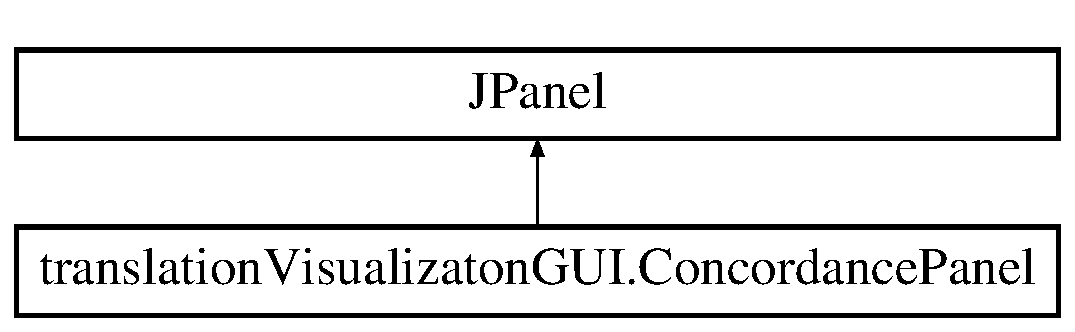
\includegraphics[height=2.000000cm]{classtranslation_visualizaton_g_u_i_1_1_concordance_panel}
\end{center}
\end{figure}
\subsection*{Public Member Functions}
\begin{DoxyCompactItemize}
\item 
\hyperlink{classtranslation_visualizaton_g_u_i_1_1_concordance_panel_af8d561bf830b8d44bc126c4cd9ed929c}{Concordance\+Panel} (List$<$ Version $>$ version\+List)
\item 
\mbox{\Hypertarget{classtranslation_visualizaton_g_u_i_1_1_concordance_panel_a538f8b21c0601fe10eb07d8d3379292c}\label{classtranslation_visualizaton_g_u_i_1_1_concordance_panel_a538f8b21c0601fe10eb07d8d3379292c}} 
boolean {\bfseries is\+First\+Version} ()
\item 
\mbox{\Hypertarget{classtranslation_visualizaton_g_u_i_1_1_concordance_panel_aac735e555a49de538d6a7213f7636da5}\label{classtranslation_visualizaton_g_u_i_1_1_concordance_panel_aac735e555a49de538d6a7213f7636da5}} 
void {\bfseries set\+First\+Version} (boolean first\+Version)
\item 
\mbox{\Hypertarget{classtranslation_visualizaton_g_u_i_1_1_concordance_panel_a3f72c6305a923b4a969bcc8cca63bc3b}\label{classtranslation_visualizaton_g_u_i_1_1_concordance_panel_a3f72c6305a923b4a969bcc8cca63bc3b}} 
boolean {\bfseries get\+M\+\_\+\+On\+And\+Off} ()
\item 
\mbox{\Hypertarget{classtranslation_visualizaton_g_u_i_1_1_concordance_panel_adf9834be2c4282c7c8c086f8d732c5e8}\label{classtranslation_visualizaton_g_u_i_1_1_concordance_panel_adf9834be2c4282c7c8c086f8d732c5e8}} 
void {\bfseries set\+On\+And\+Off} (boolean on\+And\+Off)
\item 
\mbox{\Hypertarget{classtranslation_visualizaton_g_u_i_1_1_concordance_panel_a893f9284aa2602d0f16f21315f0446ca}\label{classtranslation_visualizaton_g_u_i_1_1_concordance_panel_a893f9284aa2602d0f16f21315f0446ca}} 
int {\bfseries get\+Scale\+Value} ()
\item 
\mbox{\Hypertarget{classtranslation_visualizaton_g_u_i_1_1_concordance_panel_ac4ba5e6dddb2b4a3bccc9ddb7ca6fb35}\label{classtranslation_visualizaton_g_u_i_1_1_concordance_panel_ac4ba5e6dddb2b4a3bccc9ddb7ca6fb35}} 
void {\bfseries set\+Scale\+Value} (int scale\+Value)
\item 
\mbox{\Hypertarget{classtranslation_visualizaton_g_u_i_1_1_concordance_panel_a3d236c1a20cba529bae72c7cb5d3a83c}\label{classtranslation_visualizaton_g_u_i_1_1_concordance_panel_a3d236c1a20cba529bae72c7cb5d3a83c}} 
Data\+Reader {\bfseries get\+Data\+Reader} ()
\item 
\mbox{\Hypertarget{classtranslation_visualizaton_g_u_i_1_1_concordance_panel_a19256a3bd01d3eef77a0f402f8215585}\label{classtranslation_visualizaton_g_u_i_1_1_concordance_panel_a19256a3bd01d3eef77a0f402f8215585}} 
void {\bfseries set\+Data\+Reader} (Data\+Reader data\+Reader)
\item 
\mbox{\Hypertarget{classtranslation_visualizaton_g_u_i_1_1_concordance_panel_acfb2db1f7c233fb47da6b0f9287afea8}\label{classtranslation_visualizaton_g_u_i_1_1_concordance_panel_acfb2db1f7c233fb47da6b0f9287afea8}} 
int {\bfseries get\+M\+\_\+\+Version\+Number} ()
\item 
\mbox{\Hypertarget{classtranslation_visualizaton_g_u_i_1_1_concordance_panel_a977f192cae481bb1f15079bd4684a7d3}\label{classtranslation_visualizaton_g_u_i_1_1_concordance_panel_a977f192cae481bb1f15079bd4684a7d3}} 
void {\bfseries set\+M\+\_\+\+Version\+Number} (int m\+\_\+\+Version\+Number)
\item 
\mbox{\Hypertarget{classtranslation_visualizaton_g_u_i_1_1_concordance_panel_a707c311cab91fcd96aa0528edee5db1e}\label{classtranslation_visualizaton_g_u_i_1_1_concordance_panel_a707c311cab91fcd96aa0528edee5db1e}} 
List$<$ Version $>$ {\bfseries get\+M\+\_\+\+Version\+List} ()
\item 
\mbox{\Hypertarget{classtranslation_visualizaton_g_u_i_1_1_concordance_panel_aaa6373d0445cd90a3436138c2fc236c6}\label{classtranslation_visualizaton_g_u_i_1_1_concordance_panel_aaa6373d0445cd90a3436138c2fc236c6}} 
void {\bfseries set\+M\+\_\+\+Version\+List} (List$<$ Version $>$ \hyperlink{classtranslation_visualizaton_g_u_i_1_1_concordance_panel_a515912c3a5882d7ffad078b7cf7b614e}{m\+\_\+\+Version\+List})
\item 
\mbox{\Hypertarget{classtranslation_visualizaton_g_u_i_1_1_concordance_panel_a06e0027e952956add552659d0c12b461}\label{classtranslation_visualizaton_g_u_i_1_1_concordance_panel_a06e0027e952956add552659d0c12b461}} 
Version {\bfseries get\+M\+\_\+single\+Version} ()
\item 
\mbox{\Hypertarget{classtranslation_visualizaton_g_u_i_1_1_concordance_panel_a88c15ce838b9753178d737706a1e2b52}\label{classtranslation_visualizaton_g_u_i_1_1_concordance_panel_a88c15ce838b9753178d737706a1e2b52}} 
void {\bfseries set\+M\+\_\+single\+Version} (Version m\+\_\+single\+Version)
\item 
double \hyperlink{classtranslation_visualizaton_g_u_i_1_1_concordance_panel_a3143904a9322449a0b577194a492ede0}{get\+Zoom\+Value} ()
\item 
void \hyperlink{classtranslation_visualizaton_g_u_i_1_1_concordance_panel_a09b316adf18485d4f1c53e86b46eb780}{set\+Zoom\+Value} (int zoom\+Value)
\item 
\mbox{\Hypertarget{classtranslation_visualizaton_g_u_i_1_1_concordance_panel_a8c481564463d10e9f5e7df34479febf3}\label{classtranslation_visualizaton_g_u_i_1_1_concordance_panel_a8c481564463d10e9f5e7df34479febf3}} 
Point {\bfseries get\+Highlight\+Point} (Point event\+Point, int scale\+Value)
\item 
void \hyperlink{classtranslation_visualizaton_g_u_i_1_1_concordance_panel_af3a9707e42d94bea4d7995927bc2bbcb}{display\+Single\+Version} (List$<$ String $>$ Version\+Selected)
\item 
\mbox{\Hypertarget{classtranslation_visualizaton_g_u_i_1_1_concordance_panel_a8a77a47204bb5df44fccce3bfa1caf80}\label{classtranslation_visualizaton_g_u_i_1_1_concordance_panel_a8a77a47204bb5df44fccce3bfa1caf80}} 
void {\bfseries reset\+Locations} ()
\item 
void \hyperlink{classtranslation_visualizaton_g_u_i_1_1_concordance_panel_ae6d25eb2cfc8138b251aef627c5b488c}{scale\+Concordance\+Panel} (int scale\+Value)
\item 
void \hyperlink{classtranslation_visualizaton_g_u_i_1_1_concordance_panel_a3594f96dfd91bfcf29ce1290b1aab8a1}{freq\+Highlight} (String token)
\item 
void \hyperlink{classtranslation_visualizaton_g_u_i_1_1_concordance_panel_afded200aebb62892defa82de90b4db47}{token\+High\+Light} (Point point)
\item 
\mbox{\Hypertarget{classtranslation_visualizaton_g_u_i_1_1_concordance_panel_a80f5b7ec9dde95c9e8adeca0884af361}\label{classtranslation_visualizaton_g_u_i_1_1_concordance_panel_a80f5b7ec9dde95c9e8adeca0884af361}} 
void {\bfseries click\+Trans\+Version} (int version\+Number, int line\+Number, Version choosen\+Version, Item choosen\+Concordance)
\item 
\mbox{\Hypertarget{classtranslation_visualizaton_g_u_i_1_1_concordance_panel_a0818bca964b781800b90c5b422d39f1b}\label{classtranslation_visualizaton_g_u_i_1_1_concordance_panel_a0818bca964b781800b90c5b422d39f1b}} 
void {\bfseries click\+Base\+Text} (int version\+Number, int line\+Number, Version choosen\+Version, Item choosen\+Concordance)
\item 
void \hyperlink{classtranslation_visualizaton_g_u_i_1_1_concordance_panel_a6cf64e1636b26682080e80a25b714e78}{draw\+Title\+String} (Version version, Graphics g)
\item 
void \hyperlink{classtranslation_visualizaton_g_u_i_1_1_concordance_panel_a074ea77e057f90027a53e8782fdc3b9b}{draw\+Token\+Strings} (Graphics g)
\item 
void \hyperlink{classtranslation_visualizaton_g_u_i_1_1_concordance_panel_ad5d660a57a72f6a3966dcbf0dbb6e1a6}{draw\+Rectangles} (Graphics g)
\item 
void \hyperlink{classtranslation_visualizaton_g_u_i_1_1_concordance_panel_a3b4f98de7781aceafcb349d5763b8c38}{paint\+Component} (Graphics g)
\item 
\mbox{\Hypertarget{classtranslation_visualizaton_g_u_i_1_1_concordance_panel_a7b64ac976cb4202cd5387a0ca4b5547b}\label{classtranslation_visualizaton_g_u_i_1_1_concordance_panel_a7b64ac976cb4202cd5387a0ca4b5547b}} 
void {\bfseries draw\+Lines} (Item concordance\+Compare, Graphics g)
\item 
\mbox{\Hypertarget{classtranslation_visualizaton_g_u_i_1_1_concordance_panel_a3a0d8167ca42465228337bc03687517e}\label{classtranslation_visualizaton_g_u_i_1_1_concordance_panel_a3a0d8167ca42465228337bc03687517e}} 
boolean {\bfseries is\+Freq\+Or\+Tfidf} ()
\item 
\mbox{\Hypertarget{classtranslation_visualizaton_g_u_i_1_1_concordance_panel_a266153035b6c2415c7a40c05f4707320}\label{classtranslation_visualizaton_g_u_i_1_1_concordance_panel_a266153035b6c2415c7a40c05f4707320}} 
void {\bfseries set\+Freq\+Or\+Tfidf} (boolean freq\+Or\+Tfidf)
\item 
\mbox{\Hypertarget{classtranslation_visualizaton_g_u_i_1_1_concordance_panel_af2fd95324654f69a7802abd4e9da75ff}\label{classtranslation_visualizaton_g_u_i_1_1_concordance_panel_af2fd95324654f69a7802abd4e9da75ff}} 
Version {\bfseries get\+M\+\_\+\+Version} ()
\item 
\mbox{\Hypertarget{classtranslation_visualizaton_g_u_i_1_1_concordance_panel_af4140a6c7ee173f31db6e67e4cf4187b}\label{classtranslation_visualizaton_g_u_i_1_1_concordance_panel_af4140a6c7ee173f31db6e67e4cf4187b}} 
void {\bfseries set\+M\+\_\+\+Version} (Version m\+\_\+\+Version)
\item 
\mbox{\Hypertarget{classtranslation_visualizaton_g_u_i_1_1_concordance_panel_ab5857b6d23a2eacaf4f0ad67c35c5ca9}\label{classtranslation_visualizaton_g_u_i_1_1_concordance_panel_ab5857b6d23a2eacaf4f0ad67c35c5ca9}} 
Item {\bfseries get\+M\+\_\+\+Concordance} ()
\item 
\mbox{\Hypertarget{classtranslation_visualizaton_g_u_i_1_1_concordance_panel_a43fdfea140b513c3a9afeae865f9490e}\label{classtranslation_visualizaton_g_u_i_1_1_concordance_panel_a43fdfea140b513c3a9afeae865f9490e}} 
void {\bfseries set\+M\+\_\+\+Concordance} (Item m\+\_\+\+Concordance)
\end{DoxyCompactItemize}
\subsection*{Public Attributes}
\begin{DoxyCompactItemize}
\item 
List$<$ Version $>$ \hyperlink{classtranslation_visualizaton_g_u_i_1_1_concordance_panel_a515912c3a5882d7ffad078b7cf7b614e}{m\+\_\+\+Version\+List} =new Array\+List$<$Version$>$()
\item 
\mbox{\Hypertarget{classtranslation_visualizaton_g_u_i_1_1_concordance_panel_aa033379581a233782ae9db0cd3be89a4}\label{classtranslation_visualizaton_g_u_i_1_1_concordance_panel_aa033379581a233782ae9db0cd3be89a4}} 
boolean {\bfseries freq\+Or\+Tfidf} =false
\end{DoxyCompactItemize}


\subsection{Constructor \& Destructor Documentation}
\mbox{\Hypertarget{classtranslation_visualizaton_g_u_i_1_1_concordance_panel_af8d561bf830b8d44bc126c4cd9ed929c}\label{classtranslation_visualizaton_g_u_i_1_1_concordance_panel_af8d561bf830b8d44bc126c4cd9ed929c}} 
\index{translation\+Visualizaton\+G\+U\+I\+::\+Concordance\+Panel@{translation\+Visualizaton\+G\+U\+I\+::\+Concordance\+Panel}!Concordance\+Panel@{Concordance\+Panel}}
\index{Concordance\+Panel@{Concordance\+Panel}!translation\+Visualizaton\+G\+U\+I\+::\+Concordance\+Panel@{translation\+Visualizaton\+G\+U\+I\+::\+Concordance\+Panel}}
\subsubsection{\texorpdfstring{Concordance\+Panel()}{ConcordancePanel()}}
{\footnotesize\ttfamily translation\+Visualizaton\+G\+U\+I.\+Concordance\+Panel.\+Concordance\+Panel (\begin{DoxyParamCaption}\item[{List$<$ Version $>$}]{version\+List }\end{DoxyParamCaption})\hspace{0.3cm}{\ttfamily [inline]}}

Constructor 
\begin{DoxyParams}{Parameters}
{\em version\+List} & \\
\hline
\end{DoxyParams}


\subsection{Member Function Documentation}
\mbox{\Hypertarget{classtranslation_visualizaton_g_u_i_1_1_concordance_panel_af3a9707e42d94bea4d7995927bc2bbcb}\label{classtranslation_visualizaton_g_u_i_1_1_concordance_panel_af3a9707e42d94bea4d7995927bc2bbcb}} 
\index{translation\+Visualizaton\+G\+U\+I\+::\+Concordance\+Panel@{translation\+Visualizaton\+G\+U\+I\+::\+Concordance\+Panel}!display\+Single\+Version@{display\+Single\+Version}}
\index{display\+Single\+Version@{display\+Single\+Version}!translation\+Visualizaton\+G\+U\+I\+::\+Concordance\+Panel@{translation\+Visualizaton\+G\+U\+I\+::\+Concordance\+Panel}}
\subsubsection{\texorpdfstring{display\+Single\+Version()}{displaySingleVersion()}}
{\footnotesize\ttfamily void translation\+Visualizaton\+G\+U\+I.\+Concordance\+Panel.\+display\+Single\+Version (\begin{DoxyParamCaption}\item[{List$<$ String $>$}]{Version\+Selected }\end{DoxyParamCaption})\hspace{0.3cm}{\ttfamily [inline]}}


\begin{DoxyParams}{Parameters}
{\em List$<$\+String$>$} & \\
\hline
\end{DoxyParams}
\mbox{\Hypertarget{classtranslation_visualizaton_g_u_i_1_1_concordance_panel_ad5d660a57a72f6a3966dcbf0dbb6e1a6}\label{classtranslation_visualizaton_g_u_i_1_1_concordance_panel_ad5d660a57a72f6a3966dcbf0dbb6e1a6}} 
\index{translation\+Visualizaton\+G\+U\+I\+::\+Concordance\+Panel@{translation\+Visualizaton\+G\+U\+I\+::\+Concordance\+Panel}!draw\+Rectangles@{draw\+Rectangles}}
\index{draw\+Rectangles@{draw\+Rectangles}!translation\+Visualizaton\+G\+U\+I\+::\+Concordance\+Panel@{translation\+Visualizaton\+G\+U\+I\+::\+Concordance\+Panel}}
\subsubsection{\texorpdfstring{draw\+Rectangles()}{drawRectangles()}}
{\footnotesize\ttfamily void translation\+Visualizaton\+G\+U\+I.\+Concordance\+Panel.\+draw\+Rectangles (\begin{DoxyParamCaption}\item[{Graphics}]{g }\end{DoxyParamCaption})\hspace{0.3cm}{\ttfamily [inline]}}

Draw all the rectangles for tokens 
\begin{DoxyParams}{Parameters}
{\em g} & -\/ the Graphic to be drawed \\
\hline
\end{DoxyParams}
\mbox{\Hypertarget{classtranslation_visualizaton_g_u_i_1_1_concordance_panel_a6cf64e1636b26682080e80a25b714e78}\label{classtranslation_visualizaton_g_u_i_1_1_concordance_panel_a6cf64e1636b26682080e80a25b714e78}} 
\index{translation\+Visualizaton\+G\+U\+I\+::\+Concordance\+Panel@{translation\+Visualizaton\+G\+U\+I\+::\+Concordance\+Panel}!draw\+Title\+String@{draw\+Title\+String}}
\index{draw\+Title\+String@{draw\+Title\+String}!translation\+Visualizaton\+G\+U\+I\+::\+Concordance\+Panel@{translation\+Visualizaton\+G\+U\+I\+::\+Concordance\+Panel}}
\subsubsection{\texorpdfstring{draw\+Title\+String()}{drawTitleString()}}
{\footnotesize\ttfamily void translation\+Visualizaton\+G\+U\+I.\+Concordance\+Panel.\+draw\+Title\+String (\begin{DoxyParamCaption}\item[{Version}]{version,  }\item[{Graphics}]{g }\end{DoxyParamCaption})\hspace{0.3cm}{\ttfamily [inline]}}

Draw the stirng of titles, including author names and publish years 
\begin{DoxyParams}{Parameters}
{\em version} & -\/ current Version object \\
\hline
{\em g} & -\/ the Graphic to be drawed \\
\hline
\end{DoxyParams}
\mbox{\Hypertarget{classtranslation_visualizaton_g_u_i_1_1_concordance_panel_a074ea77e057f90027a53e8782fdc3b9b}\label{classtranslation_visualizaton_g_u_i_1_1_concordance_panel_a074ea77e057f90027a53e8782fdc3b9b}} 
\index{translation\+Visualizaton\+G\+U\+I\+::\+Concordance\+Panel@{translation\+Visualizaton\+G\+U\+I\+::\+Concordance\+Panel}!draw\+Token\+Strings@{draw\+Token\+Strings}}
\index{draw\+Token\+Strings@{draw\+Token\+Strings}!translation\+Visualizaton\+G\+U\+I\+::\+Concordance\+Panel@{translation\+Visualizaton\+G\+U\+I\+::\+Concordance\+Panel}}
\subsubsection{\texorpdfstring{draw\+Token\+Strings()}{drawTokenStrings()}}
{\footnotesize\ttfamily void translation\+Visualizaton\+G\+U\+I.\+Concordance\+Panel.\+draw\+Token\+Strings (\begin{DoxyParamCaption}\item[{Graphics}]{g }\end{DoxyParamCaption})\hspace{0.3cm}{\ttfamily [inline]}}

Draw token strings 
\begin{DoxyParams}{Parameters}
{\em g} & -\/ the Graphic to be drawed \\
\hline
\end{DoxyParams}
\mbox{\Hypertarget{classtranslation_visualizaton_g_u_i_1_1_concordance_panel_a3594f96dfd91bfcf29ce1290b1aab8a1}\label{classtranslation_visualizaton_g_u_i_1_1_concordance_panel_a3594f96dfd91bfcf29ce1290b1aab8a1}} 
\index{translation\+Visualizaton\+G\+U\+I\+::\+Concordance\+Panel@{translation\+Visualizaton\+G\+U\+I\+::\+Concordance\+Panel}!freq\+Highlight@{freq\+Highlight}}
\index{freq\+Highlight@{freq\+Highlight}!translation\+Visualizaton\+G\+U\+I\+::\+Concordance\+Panel@{translation\+Visualizaton\+G\+U\+I\+::\+Concordance\+Panel}}
\subsubsection{\texorpdfstring{freq\+Highlight()}{freqHighlight()}}
{\footnotesize\ttfamily void translation\+Visualizaton\+G\+U\+I.\+Concordance\+Panel.\+freq\+Highlight (\begin{DoxyParamCaption}\item[{String}]{token }\end{DoxyParamCaption})\hspace{0.3cm}{\ttfamily [inline]}}

if one color on color legend panel is clicked, all tokens with the ame frequency will be highlighted 
\begin{DoxyParams}{Parameters}
{\em token} & \\
\hline
\end{DoxyParams}
\mbox{\Hypertarget{classtranslation_visualizaton_g_u_i_1_1_concordance_panel_a3143904a9322449a0b577194a492ede0}\label{classtranslation_visualizaton_g_u_i_1_1_concordance_panel_a3143904a9322449a0b577194a492ede0}} 
\index{translation\+Visualizaton\+G\+U\+I\+::\+Concordance\+Panel@{translation\+Visualizaton\+G\+U\+I\+::\+Concordance\+Panel}!get\+Zoom\+Value@{get\+Zoom\+Value}}
\index{get\+Zoom\+Value@{get\+Zoom\+Value}!translation\+Visualizaton\+G\+U\+I\+::\+Concordance\+Panel@{translation\+Visualizaton\+G\+U\+I\+::\+Concordance\+Panel}}
\subsubsection{\texorpdfstring{get\+Zoom\+Value()}{getZoomValue()}}
{\footnotesize\ttfamily double translation\+Visualizaton\+G\+U\+I.\+Concordance\+Panel.\+get\+Zoom\+Value (\begin{DoxyParamCaption}{ }\end{DoxyParamCaption})\hspace{0.3cm}{\ttfamily [inline]}}

a formula is applied here to make sure we return a float value to fit the .scale() method. \begin{DoxyReturn}{Returns}
zoom\+Value 
\end{DoxyReturn}
\mbox{\Hypertarget{classtranslation_visualizaton_g_u_i_1_1_concordance_panel_a3b4f98de7781aceafcb349d5763b8c38}\label{classtranslation_visualizaton_g_u_i_1_1_concordance_panel_a3b4f98de7781aceafcb349d5763b8c38}} 
\index{translation\+Visualizaton\+G\+U\+I\+::\+Concordance\+Panel@{translation\+Visualizaton\+G\+U\+I\+::\+Concordance\+Panel}!paint\+Component@{paint\+Component}}
\index{paint\+Component@{paint\+Component}!translation\+Visualizaton\+G\+U\+I\+::\+Concordance\+Panel@{translation\+Visualizaton\+G\+U\+I\+::\+Concordance\+Panel}}
\subsubsection{\texorpdfstring{paint\+Component()}{paintComponent()}}
{\footnotesize\ttfamily void translation\+Visualizaton\+G\+U\+I.\+Concordance\+Panel.\+paint\+Component (\begin{DoxyParamCaption}\item[{Graphics}]{g }\end{DoxyParamCaption})\hspace{0.3cm}{\ttfamily [inline]}}

Draw the version visualization on \hyperlink{classtranslation_visualizaton_g_u_i_1_1_concordance_panel}{Concordance\+Panel}. This method is called from \hyperlink{classtranslation_visualizaton_g_u_i_1_1_concordance_panel}{Concordance\+Panel}. \mbox{\Hypertarget{classtranslation_visualizaton_g_u_i_1_1_concordance_panel_ae6d25eb2cfc8138b251aef627c5b488c}\label{classtranslation_visualizaton_g_u_i_1_1_concordance_panel_ae6d25eb2cfc8138b251aef627c5b488c}} 
\index{translation\+Visualizaton\+G\+U\+I\+::\+Concordance\+Panel@{translation\+Visualizaton\+G\+U\+I\+::\+Concordance\+Panel}!scale\+Concordance\+Panel@{scale\+Concordance\+Panel}}
\index{scale\+Concordance\+Panel@{scale\+Concordance\+Panel}!translation\+Visualizaton\+G\+U\+I\+::\+Concordance\+Panel@{translation\+Visualizaton\+G\+U\+I\+::\+Concordance\+Panel}}
\subsubsection{\texorpdfstring{scale\+Concordance\+Panel()}{scaleConcordancePanel()}}
{\footnotesize\ttfamily void translation\+Visualizaton\+G\+U\+I.\+Concordance\+Panel.\+scale\+Concordance\+Panel (\begin{DoxyParamCaption}\item[{int}]{scale\+Value }\end{DoxyParamCaption})\hspace{0.3cm}{\ttfamily [inline]}}

rescale concordance panel, recalculate the locations and widths 
\begin{DoxyParams}{Parameters}
{\em scale\+Value} & \\
\hline
\end{DoxyParams}
\mbox{\Hypertarget{classtranslation_visualizaton_g_u_i_1_1_concordance_panel_a09b316adf18485d4f1c53e86b46eb780}\label{classtranslation_visualizaton_g_u_i_1_1_concordance_panel_a09b316adf18485d4f1c53e86b46eb780}} 
\index{translation\+Visualizaton\+G\+U\+I\+::\+Concordance\+Panel@{translation\+Visualizaton\+G\+U\+I\+::\+Concordance\+Panel}!set\+Zoom\+Value@{set\+Zoom\+Value}}
\index{set\+Zoom\+Value@{set\+Zoom\+Value}!translation\+Visualizaton\+G\+U\+I\+::\+Concordance\+Panel@{translation\+Visualizaton\+G\+U\+I\+::\+Concordance\+Panel}}
\subsubsection{\texorpdfstring{set\+Zoom\+Value()}{setZoomValue()}}
{\footnotesize\ttfamily void translation\+Visualizaton\+G\+U\+I.\+Concordance\+Panel.\+set\+Zoom\+Value (\begin{DoxyParamCaption}\item[{int}]{zoom\+Value }\end{DoxyParamCaption})\hspace{0.3cm}{\ttfamily [inline]}}

this method pass zoom\+Value from translation\+Visualization.\+get\+M\+\_\+\+Slider().add\+Change\+Listener() 
\begin{DoxyParams}{Parameters}
{\em scale\+Value} & \\
\hline
\end{DoxyParams}
\mbox{\Hypertarget{classtranslation_visualizaton_g_u_i_1_1_concordance_panel_afded200aebb62892defa82de90b4db47}\label{classtranslation_visualizaton_g_u_i_1_1_concordance_panel_afded200aebb62892defa82de90b4db47}} 
\index{translation\+Visualizaton\+G\+U\+I\+::\+Concordance\+Panel@{translation\+Visualizaton\+G\+U\+I\+::\+Concordance\+Panel}!token\+High\+Light@{token\+High\+Light}}
\index{token\+High\+Light@{token\+High\+Light}!translation\+Visualizaton\+G\+U\+I\+::\+Concordance\+Panel@{translation\+Visualizaton\+G\+U\+I\+::\+Concordance\+Panel}}
\subsubsection{\texorpdfstring{token\+High\+Light()}{tokenHighLight()}}
{\footnotesize\ttfamily void translation\+Visualizaton\+G\+U\+I.\+Concordance\+Panel.\+token\+High\+Light (\begin{DoxyParamCaption}\item[{Point}]{point }\end{DoxyParamCaption})\hspace{0.3cm}{\ttfamily [inline]}}

set the transparency of the rectangles\textquotesingle{} when one token is clicked 
\begin{DoxyParams}{Parameters}
{\em point} & \\
\hline
\end{DoxyParams}


\subsection{Member Data Documentation}
\mbox{\Hypertarget{classtranslation_visualizaton_g_u_i_1_1_concordance_panel_a515912c3a5882d7ffad078b7cf7b614e}\label{classtranslation_visualizaton_g_u_i_1_1_concordance_panel_a515912c3a5882d7ffad078b7cf7b614e}} 
\index{translation\+Visualizaton\+G\+U\+I\+::\+Concordance\+Panel@{translation\+Visualizaton\+G\+U\+I\+::\+Concordance\+Panel}!m\+\_\+\+Version\+List@{m\+\_\+\+Version\+List}}
\index{m\+\_\+\+Version\+List@{m\+\_\+\+Version\+List}!translation\+Visualizaton\+G\+U\+I\+::\+Concordance\+Panel@{translation\+Visualizaton\+G\+U\+I\+::\+Concordance\+Panel}}
\subsubsection{\texorpdfstring{m\+\_\+\+Version\+List}{m\_VersionList}}
{\footnotesize\ttfamily List$<$Version$>$ translation\+Visualizaton\+G\+U\+I.\+Concordance\+Panel.\+m\+\_\+\+Version\+List =new Array\+List$<$Version$>$()}

the list of versions passed from translation visualization 

The documentation for this class was generated from the following file\+:\begin{DoxyCompactItemize}
\item 
Concordance\+Panel.\+java\end{DoxyCompactItemize}

\hypertarget{classtranslation_visualizaton_g_u_i_1_1_version_chosen_panel}{}\section{translation\+Visualizaton\+G\+U\+I.\+Version\+Chosen\+Panel Class Reference}
\label{classtranslation_visualizaton_g_u_i_1_1_version_chosen_panel}\index{translation\+Visualizaton\+G\+U\+I.\+Version\+Chosen\+Panel@{translation\+Visualizaton\+G\+U\+I.\+Version\+Chosen\+Panel}}
Inheritance diagram for translation\+Visualizaton\+G\+U\+I.\+Version\+Chosen\+Panel\+:\begin{figure}[H]
\begin{center}
\leavevmode
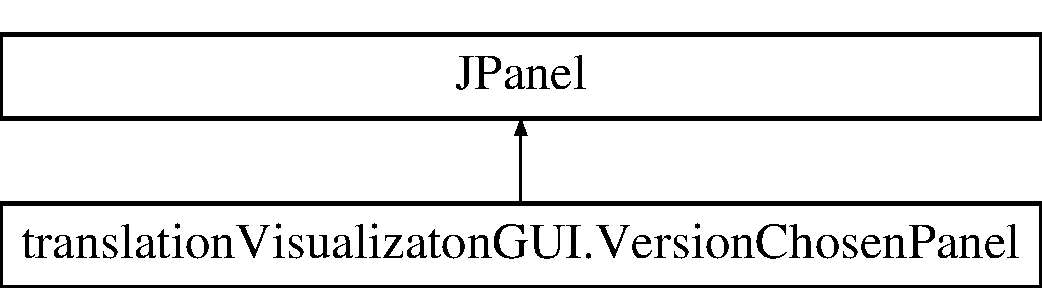
\includegraphics[height=2.000000cm]{classtranslation_visualizaton_g_u_i_1_1_version_chosen_panel}
\end{center}
\end{figure}
\subsection*{Public Member Functions}
\begin{DoxyCompactItemize}
\item 
String \mbox{[}$\,$\mbox{]} \hyperlink{classtranslation_visualizaton_g_u_i_1_1_version_chosen_panel_a8b960328c36ce36d4817837bd0843f9c}{get\+M\+\_\+\+File\+Path} ()
\item 
\mbox{\Hypertarget{classtranslation_visualizaton_g_u_i_1_1_version_chosen_panel_a1a894cf67cc38c7e8ba7a94c432903bf}\label{classtranslation_visualizaton_g_u_i_1_1_version_chosen_panel_a1a894cf67cc38c7e8ba7a94c432903bf}} 
void {\bfseries set\+Initial\+File\+Path} ()
\item 
\mbox{\Hypertarget{classtranslation_visualizaton_g_u_i_1_1_version_chosen_panel_a9f46f0beb66850276b0a72df287c2c03}\label{classtranslation_visualizaton_g_u_i_1_1_version_chosen_panel_a9f46f0beb66850276b0a72df287c2c03}} 
void {\bfseries set\+German\+Lemma\+File\+Path} ()
\item 
\mbox{\Hypertarget{classtranslation_visualizaton_g_u_i_1_1_version_chosen_panel_a83db8b074f9bdb726ffe7d383a440d2d}\label{classtranslation_visualizaton_g_u_i_1_1_version_chosen_panel_a83db8b074f9bdb726ffe7d383a440d2d}} 
void {\bfseries add\+All\+Versions} (String\mbox{[}$\,$\mbox{]} string)
\item 
\mbox{\Hypertarget{classtranslation_visualizaton_g_u_i_1_1_version_chosen_panel_a2c0bd0472fd45a69755ee270a5cca0a2}\label{classtranslation_visualizaton_g_u_i_1_1_version_chosen_panel_a2c0bd0472fd45a69755ee270a5cca0a2}} 
List$<$ String $>$ {\bfseries get\+M\+\_\+version\+Names} ()
\item 
\mbox{\Hypertarget{classtranslation_visualizaton_g_u_i_1_1_version_chosen_panel_aae3a8d811c19be05919c37607c92945f}\label{classtranslation_visualizaton_g_u_i_1_1_version_chosen_panel_aae3a8d811c19be05919c37607c92945f}} 
void {\bfseries set\+M\+\_\+version\+Names} (List$<$ String $>$ \hyperlink{classtranslation_visualizaton_g_u_i_1_1_version_chosen_panel_a886df3a3c3c1d8bd15320d84972fa518}{m\+\_\+version\+Names})
\item 
\mbox{\Hypertarget{classtranslation_visualizaton_g_u_i_1_1_version_chosen_panel_ae07211a76c075a6ec4eb081a6a5ca810}\label{classtranslation_visualizaton_g_u_i_1_1_version_chosen_panel_ae07211a76c075a6ec4eb081a6a5ca810}} 
List$<$ J\+Check\+Box $>$ {\bfseries get\+M\+\_\+check\+List} ()
\item 
\mbox{\Hypertarget{classtranslation_visualizaton_g_u_i_1_1_version_chosen_panel_ab65ec963122aac458976889690c0e89e}\label{classtranslation_visualizaton_g_u_i_1_1_version_chosen_panel_ab65ec963122aac458976889690c0e89e}} 
void {\bfseries set\+M\+\_\+check\+List} (List$<$ J\+Check\+Box $>$ m\+\_\+check\+List)
\item 
\mbox{\Hypertarget{classtranslation_visualizaton_g_u_i_1_1_version_chosen_panel_a7216d96540ef92e6f03f7325662800a4}\label{classtranslation_visualizaton_g_u_i_1_1_version_chosen_panel_a7216d96540ef92e6f03f7325662800a4}} 
J\+Check\+Box {\bfseries get\+M\+\_\+\+Version\+Name\+C\+Box} ()
\item 
\mbox{\Hypertarget{classtranslation_visualizaton_g_u_i_1_1_version_chosen_panel_ab932a10c31253adef07f95e1b12c1f1a}\label{classtranslation_visualizaton_g_u_i_1_1_version_chosen_panel_ab932a10c31253adef07f95e1b12c1f1a}} 
void {\bfseries set\+M\+\_\+\+Version\+Name\+C\+Box} (J\+Check\+Box m\+\_\+\+Version\+Name\+C\+Box, String str)
\item 
\mbox{\Hypertarget{classtranslation_visualizaton_g_u_i_1_1_version_chosen_panel_a65890ec34a6b133b8678b856f7264d92}\label{classtranslation_visualizaton_g_u_i_1_1_version_chosen_panel_a65890ec34a6b133b8678b856f7264d92}} 
void {\bfseries all\+Selection} (Action\+Event action\+Event, \hyperlink{classtranslation_visualizaton_g_u_i_1_1_concordance_panel}{Concordance\+Panel} concordance\+Panel)
\item 
\mbox{\Hypertarget{classtranslation_visualizaton_g_u_i_1_1_version_chosen_panel_abadb59898059cde97ede15236b35c6f9}\label{classtranslation_visualizaton_g_u_i_1_1_version_chosen_panel_abadb59898059cde97ede15236b35c6f9}} 
void {\bfseries single\+Selection} (Action\+Event action\+Event, \hyperlink{classtranslation_visualizaton_g_u_i_1_1_concordance_panel}{Concordance\+Panel} concordance\+Panel, Boolean one\+Selected)
\item 
\mbox{\Hypertarget{classtranslation_visualizaton_g_u_i_1_1_version_chosen_panel_a513fc68c9445556bb641d406e2dd4beb}\label{classtranslation_visualizaton_g_u_i_1_1_version_chosen_panel_a513fc68c9445556bb641d406e2dd4beb}} 
Action\+Listener {\bfseries add\+\_\+\+Action\+Listener} (\hyperlink{classtranslation_visualizaton_g_u_i_1_1_concordance_panel}{Concordance\+Panel} concordance\+Panel)
\item 
\mbox{\Hypertarget{classtranslation_visualizaton_g_u_i_1_1_version_chosen_panel_a8fd52f796bf4485a6ed62d4e7b8560eb}\label{classtranslation_visualizaton_g_u_i_1_1_version_chosen_panel_a8fd52f796bf4485a6ed62d4e7b8560eb}} 
void {\bfseries add\+Versions} (List$<$ String $>$ version\+Name\+List, \hyperlink{classtranslation_visualizaton_g_u_i_1_1_concordance_panel}{Concordance\+Panel} concordance\+Panel)
\item 
\mbox{\Hypertarget{classtranslation_visualizaton_g_u_i_1_1_version_chosen_panel_a7622fd698b62bba1108d63b193a6e024}\label{classtranslation_visualizaton_g_u_i_1_1_version_chosen_panel_a7622fd698b62bba1108d63b193a6e024}} 
void {\bfseries initialize} (\hyperlink{classtranslation_visualizaton_g_u_i_1_1_concordance_panel}{Concordance\+Panel} concordance\+Panel, List$<$ String $>$ version\+Names)
\item 
\mbox{\Hypertarget{classtranslation_visualizaton_g_u_i_1_1_version_chosen_panel_a0225922f91d4b05d7bec64921df05e07}\label{classtranslation_visualizaton_g_u_i_1_1_version_chosen_panel_a0225922f91d4b05d7bec64921df05e07}} 
Grid\+Bag\+Constraints {\bfseries get\+Constraint} ()
\end{DoxyCompactItemize}
\subsection*{Public Attributes}
\begin{DoxyCompactItemize}
\item 
List$<$ String $>$ \hyperlink{classtranslation_visualizaton_g_u_i_1_1_version_chosen_panel_a886df3a3c3c1d8bd15320d84972fa518}{m\+\_\+version\+Names}
\item 
String \mbox{[}$\,$\mbox{]} {\bfseries m\+\_\+\+File\+Path}
\end{DoxyCompactItemize}


\subsection{Member Function Documentation}
\mbox{\Hypertarget{classtranslation_visualizaton_g_u_i_1_1_version_chosen_panel_a8b960328c36ce36d4817837bd0843f9c}\label{classtranslation_visualizaton_g_u_i_1_1_version_chosen_panel_a8b960328c36ce36d4817837bd0843f9c}} 
\index{translation\+Visualizaton\+G\+U\+I\+::\+Version\+Chosen\+Panel@{translation\+Visualizaton\+G\+U\+I\+::\+Version\+Chosen\+Panel}!get\+M\+\_\+\+File\+Path@{get\+M\+\_\+\+File\+Path}}
\index{get\+M\+\_\+\+File\+Path@{get\+M\+\_\+\+File\+Path}!translation\+Visualizaton\+G\+U\+I\+::\+Version\+Chosen\+Panel@{translation\+Visualizaton\+G\+U\+I\+::\+Version\+Chosen\+Panel}}
\subsubsection{\texorpdfstring{get\+M\+\_\+\+File\+Path()}{getM\_FilePath()}}
{\footnotesize\ttfamily String \mbox{[}$\,$\mbox{]} translation\+Visualizaton\+G\+U\+I.\+Version\+Chosen\+Panel.\+get\+M\+\_\+\+File\+Path (\begin{DoxyParamCaption}{ }\end{DoxyParamCaption})\hspace{0.3cm}{\ttfamily [inline]}}

\begin{DoxyReturn}{Returns}
file path string array 
\end{DoxyReturn}


\subsection{Member Data Documentation}
\mbox{\Hypertarget{classtranslation_visualizaton_g_u_i_1_1_version_chosen_panel_afde1444266b2eccb015a29fb5fe66b89}\label{classtranslation_visualizaton_g_u_i_1_1_version_chosen_panel_afde1444266b2eccb015a29fb5fe66b89}} 
\index{translation\+Visualizaton\+G\+U\+I\+::\+Version\+Chosen\+Panel@{translation\+Visualizaton\+G\+U\+I\+::\+Version\+Chosen\+Panel}!m\+\_\+\+File\+Path@{m\+\_\+\+File\+Path}}
\index{m\+\_\+\+File\+Path@{m\+\_\+\+File\+Path}!translation\+Visualizaton\+G\+U\+I\+::\+Version\+Chosen\+Panel@{translation\+Visualizaton\+G\+U\+I\+::\+Version\+Chosen\+Panel}}
\subsubsection{\texorpdfstring{m\+\_\+\+File\+Path}{m\_FilePath}}
{\footnotesize\ttfamily String \mbox{[}$\,$\mbox{]} translation\+Visualizaton\+G\+U\+I.\+Version\+Chosen\+Panel.\+m\+\_\+\+File\+Path}

{\bfseries Initial value\+:}
\begin{DoxyCode}
=\{ \textcolor{stringliteral}{"1604 BaseText Shakespeare.txt"}, \textcolor{stringliteral}{"1832 Baudissin ed Wenig.txt"}, \textcolor{stringliteral}{"1920 Gundolf.txt"}, \textcolor{stringliteral}{"1941 Schwarz.txt"},
            \textcolor{stringliteral}{"1947 Baudissin ed Brunner.txt"},    \textcolor{stringliteral}{"1952 Flatter.txt"}, \textcolor{stringliteral}{"1962 Schroeder.txt"},
            \textcolor{stringliteral}{"1963 Rothe.txt"}, \textcolor{stringliteral}{"1970 Fried.txt"}, \textcolor{stringliteral}{"1973 Lauterbach.txt"},
            \textcolor{stringliteral}{"1976 Engler.txt"}, \textcolor{stringliteral}{"1978 Laube.txt"}, \textcolor{stringliteral}{"1985 Bolte Hamblock.txt"},
            \textcolor{stringliteral}{"1992 Motschach.txt"}, \textcolor{stringliteral}{"1995 Guenther.txt"}, \textcolor{stringliteral}{"2003 Zaimoglu.txt"} \}
\end{DoxyCode}
\mbox{\Hypertarget{classtranslation_visualizaton_g_u_i_1_1_version_chosen_panel_a886df3a3c3c1d8bd15320d84972fa518}\label{classtranslation_visualizaton_g_u_i_1_1_version_chosen_panel_a886df3a3c3c1d8bd15320d84972fa518}} 
\index{translation\+Visualizaton\+G\+U\+I\+::\+Version\+Chosen\+Panel@{translation\+Visualizaton\+G\+U\+I\+::\+Version\+Chosen\+Panel}!m\+\_\+version\+Names@{m\+\_\+version\+Names}}
\index{m\+\_\+version\+Names@{m\+\_\+version\+Names}!translation\+Visualizaton\+G\+U\+I\+::\+Version\+Chosen\+Panel@{translation\+Visualizaton\+G\+U\+I\+::\+Version\+Chosen\+Panel}}
\subsubsection{\texorpdfstring{m\+\_\+version\+Names}{m\_versionNames}}
{\footnotesize\ttfamily List$<$String$>$ translation\+Visualizaton\+G\+U\+I.\+Version\+Chosen\+Panel.\+m\+\_\+version\+Names}

the list of String to store version names and pass this list to concordance panel and repaint new panel with versions only selected 

The documentation for this class was generated from the following file\+:\begin{DoxyCompactItemize}
\item 
Version\+Chosen\+Panel.\+java\end{DoxyCompactItemize}

%--- End generated contents ---

% Index
\backmatter
\newpage
\phantomsection
\clearemptydoublepage
\addcontentsline{toc}{chapter}{Index}
\printindex

\end{document}
